\documentclass{article}

\usepackage{pdfpages}
\usepackage{graphicx}
\usepackage[export]{adjustbox}
\usepackage{tabu}
\usepackage{xcolor,colortbl}

\begin{document}

\vspace*{3ex}
\begin{flushright}
{\large 3 March 2015}
\end{flushright}

\begin{flushleft}
{\large Jakub Ciecierski\\

}
\end{flushleft}

\hskip3cm

\begin{center}

\Large {\bf
	Cellular automaton
}

\Large {\bf 
	Requirement specification 
}

\vskip2ex

\vspace{60pt}

\includegraphics[width=80mm]{images/mini.png} \\
\end{center}

\vskip20ex

\newpage
\tableofcontents
\newpage
\section{Schedule} \par

\begin{center}

	\begin{tabular}{| l | p{7cm} |}

		\hline
		\cellcolor[HTML]{C0C0C0}Date & \cellcolor[HTML]{C0C0C0} Asset \\
		
		\hline
	  	2015-04-02 & Technical project \\
		
		\hline
	  	2015-04-23 & Code of modules\\
	
		\hline
		2015-04-30 & version 0.98\\

		\hline
		2015-05-07 & version 0.99\\	
		
		\hline
		2015-05-14 & version 1.00\\
		
		\hline
		2015-05-28 & Test report\\
		
		\hline
		2015-06-11 & Acceptation \\
		
		\hline
	
	\end{tabular}

\end{center}

\section{Document metric}


\begin{table}[h]
\hspace*{-3.1cm}
\large
\begin{tabular}{|
>{\columncolor[HTML]{C0C0C0}}l |l|l|l|l|l|}
\hline
\multicolumn{6}{|l|}{\cellcolor[HTML]{C0C0C0}Document metric}                                                                                                                                         \\ \hline
Project:       & Cellular Automaton                                                       & \cellcolor[HTML]{C0C0C0}Company: & \multicolumn{3}{l|}{WUT}                                               \\ \hline
Name:          & \multicolumn{5}{l|}{Requirement specification}                                                                                                                                       \\ \hline
Topics:        & \multicolumn{5}{l|}{Business analysis of the product}                                                                                                                                       \\ \hline
Author:        & \multicolumn{5}{l|}{Jakub Ciecierski}                                                                                                                                                \\ \hline
File:          & \multicolumn{5}{l|}{requirement\_specification.pdf}                                                                                                                                      \\ \hline
Version no:    & 0.1                                                                      & \cellcolor[HTML]{C0C0C0}Status:  & Under development & \cellcolor[HTML]{C0C0C0}Opening date: & 2015-03-03 \\ \hline
Summary:       & \multicolumn{5}{l|}{Business analysis of application that allows for creating a cellular automaton}                                                                                                           \\ \hline
Authorized by: & \begin{tabular}[c]{@{}l@{}}Władysław Homenda\\ Lucjan Stapp\end{tabular} & \multicolumn{3}{l|}{\cellcolor[HTML]{C0C0C0}Last modification date:}                         & 2015-03-03 \\ \hline
\end{tabular}
\end{table}



\section{History of changes}

\begin{table}[h]
\hspace*{-2.1cm}
\large
\begin{tabular}{|l|l|l|l|}
\hline
\multicolumn{4}{|l|}{\cellcolor[HTML]{C0C0C0}History of Changes} \\ \hline
Version         & Date         & Who        & Description        \\ \hline
0.1         & 2015-03-03         & Jakub Ciecierski        & Definition of the main purpose of the document       \\ \hline
\end{tabular}
\end{table}

\newpage
\section{Glossary} \par


\setlength{\parindent}{5ex}
\Large {\bf \hspace{15pt} Cellular automaton } - consists of a \textit{grid} of \textit{cells}, each in one of a finite number of \textit{states} (e.g. on and off). 
	A new \textit{generation} is created, according to some fixed
	\textit{rule} that determines the new state of each cell. \\


\Large {\bf 
	Cell 
}	
	- can be in one of many states,
	in case of binary cellular automaton we only have two states for each cell, namely on and off.
	For each cell, a set of cells called its
	\textit{neighborhood} is defined relative to that cell.	\\


\Large {\bf 
	Grid
} 	
	- can be in any finite number of dimensions. Consists of cells.
	An initial state is selected by assigning a state for each cell \\


\Large {\bf Rule
} 
	- determines the new state of each cell in terms of the current state
	of the cell and the states of the cells in its neighborhood.
	Typically, the rule for updating the state of cells is the same for each
	cell, and is applied to the whole grid simultaneously, such application of
	a rule to the entire grid, creates a new \textit{generation} \\

\newpage	

\Large {\bf Neighborhood
} 
	-  have possibility to introduce rules which determine the new state of 
	each cell. The transition of a cell is based on the states of his neighbors which are
	defined under different environments such as:
	\begin{itemize}
	
	\item	
		4 points neighborhood \hspace{35pt} 
			 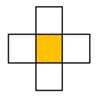
\includegraphics[width=20mm]{images/4_neigh.png} \\

	\item	
		8 points neighborhood \hspace{35pt}
			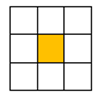
\includegraphics[width=20mm]{images/8_neigh.png} \\

	\item	
		24 points neighborhood \hspace{35pt}
			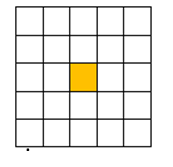
\includegraphics[width=20mm]{images/24_neigh.png} \\				
	\end{itemize}

\Large {\bf Pattern
} - is a combination of specific layout of cells on the grid and the set of rules to be applied for them.

\newpage

\section{Goal}

\hspace{15pt}The goal of this project is to create an application for cellular automaton. The automaton will consist of grid of cells that can be in either of two states
(e.i. on / off) and will operate in 3 different environments:
\begin{itemize}
	\item 4 points neighborhood.
	\item 8 points neighborhood.
	\item 24 points neighborhood.
\end{itemize}

\par The application will allow user to create, save and edit rules based on this environments and of course observe each generation on the two dimensional finite in size grid of cells
(the grid will have wrapping option to simulate infinite size - the left edge will be connected with right edge).

\par The user will be able to draw cells on the grid and save the state of grid into patterns.
The user can easily move around the grid, zoom in and out.

\newpage
\section{User stories}
	\hspace{15pt} {\bf Grid editor}
\begin{itemize}	
	\item 
		As a user, 
		I want to open grid editor,
		in order to change the grid size.

	\item 
		As a user, 
		I want to open grid editor,
		in order to change color of each state of a cell.

	\item 
		As a user, 
		I want to open grid editor,
		in order to enable/disable wrapping option.

	\item 
		As a user, 
		I want to scroll my mouse roll over the grid,
		in order to adjust the scale of the grid.

	\item 
		As a user, 
		I want to select the brush,
		in order to draw cells on the grid.

	\vspace{30pt}
	Rule editor
	
	\item 
		As a user,
		I want to open rule editor,
		in order to create new rule.
		
	\item 
		As a user,
		I want to choose neighborhood environment,
		in order to add new rule.
		
	\item 
		As a user,
		I want to define specific transition for a given state of cell,
		in order to generate new state.
		
	\item 
		As a user,
		I want to click save/save as button in rule editor,
		in order to save current rule.

	\item 
		As a user,
		I want to click load button in rule editor,
		in order to load current rule and possible edit it.

	\vspace{30pt}
	Application option
	
	\item 
		As a user,
		I want to move View components (e.g. rule editor / grid editor / browser),
		in order to position them in different location.
	\item 
		As a user,
		I want to click next generation button 
		to compute next generation
	\item 
		As a user,
		I want to click next N generations button,
		to compute next N generations.
	\item 
		As a user,
		I want to set the number of generation to skip by clicking next N generations button,
		in order to compute next N generations.
	\item 
		As a user,
		I want set the speed of computation of next generation in running mode,
		to customize the speed of which the automaton is transitioning. \\
		
		Pattern editor
	\item 
		As a user,
		I want to save a current state of grid into a pattern,
		so that later I can load it into the program.

	\item 
		As a user,
		I want to browse for my patterns in the browser window,
		in order to load it to the pattern editor.

	\item 
		As a user,
		I want to click change rule in the pattern editor,
		in order to add a rule of my choosing to that pattern.
		
\end{itemize}

\newpage

\section{Functional Requirements}
Priority
\begin{itemize} 
\item 1 - must be implemented
\item 2 - can be implemented optionally 
\item 3 - is a nice addition, but not needed.
\end{itemize} 

\begin{center}
\hspace*{-2.1cm}
	\begin{tabular}{| l | p{7cm} | p{5cm} | l |}
	
		\hline
	  	ID & Requirement & Comments & Priority \\
		\hline
		
		1 & 
		The system provides a Grid options
		allowing for changing the size, colour of cells and
		enabling/disabling wrapping option&
		The colour of cells represent a state of the cell.
		In other words the user can choose in what state to put a cell into. &
		1 
		\\ \hline

		1.1 & 
		The system should allow grid maneuvers, zooming in/out and if the
		entire grid is not visible in one screen, possibility of moving around the grid&
		 &
		1 
		\\ \hline

		2 & 
		The system provides a Rule editor in which
		the user can create, edit and save rules. & 
		 &
		1 
		\\ \hline
		
		2.1 & 
		By clicking create rule button in Rule editor, the application will open a fresh rule
		creation window & 
		 &
		1 
		\\ \hline

		2.2 & 
		By clicking load button in Rule editor, the application will open a browser which
		will allow the user to find saved rules & 
		 &
		1 
		\\ \hline

		2.3 & 
		By clicking save button in Rule editor, the application will make sure that name for the
		rule is provided and then will save the rule in specified by the user location & 
		 &
		1 

		\\ \hline


	  \hline
	\end{tabular}
\hspace*{-2.1cm}
	\begin{tabular}{| l | p{7cm} | p{5cm} | l |}
		\hline
	  	ID & Requirement & Comments & Priority \\
		\hline

		2.4 & 
		The system provides three different neighborhood environments
		in which the user can create rules, 4-point, 8-point, 24-point  & 
		See Glossary / Neighborhood for more information &
		1 
		\\ \hline
		

		2.5 & 
		The application provides special file extension for saving and keeping rules & 
		 &
		1 
		\\ \hline
				
		2.6 &
		For 4-point and 8-point environments the system should provide a way to create rules
		in which positions of neighbors relative to the cell are considered. If
		a transition is not defined then this transition does not change the state of current cell
		 &
		The user can choose to what state current cell transitions, based on this cell's state 
		and states of his neighbors &
		1 
		\\ \hline

		2.7 &
		For 24-point environment system should provide a may of creating rules in which 
		the user specifies number of neighbors in each column
		&	
		This environment can be represented as a 5 by 5 matrix with the current cell in the middle &
		1 
		\\ \hline

		2.8 &
		For 4-point, 8-point and 24-point environments the system should provide a simplified
		mode of creating rules in which the user inputs only number of neighbors in given state
		in the neighborhood for a current cell state. &
		The user inputs number of neighbors with given state which should appear for the
		cell to transition to another specified state &
		2 
		\\ \hline
				
		3.1 & 
		The system provides a step-by-step button which computes next generation & 
		 &
		1 

		\\ \hline



	\end{tabular}
\hspace*{-2.1cm}
	\begin{tabular}{| l | p{7cm} | p{5cm} | l |}
		\hline
	  	ID & Requirement & Comments & Priority \\
		 \hline

		3.2 & 
		The system provides next-N button which computes next N generations,
		the N must be easily chosen by the user & 
	 		&
		1
		\\ \hline

		3.3 & 
		The system provides a run button which will
		start the animation of consecutive generations & 
		 &
		1
		\\ \hline
		
		3.4 & 
		The system provides way to change speed of which the animation is drawn in the 'run' mode & 
		 &
		1
		\\ \hline

		4.1 & 
		The application allow user to draw cells on the grid & 
		 &
		1
		\\ \hline		

		4.2 & 
		The application provides a way for user to save grid state into patterns, additionally
		the pattern can have a rule attached to it, which later can be loaded into the grid.  & 
		A pattern editor view component should be created.
		The grid state consists of its size, states of cells and other grid options.&
		2
		\\ \hline				

		4.3 & 
		The application provides Browser window in which the 
		user can browse saved rules and patterns & 
		 &
		1 
		\\ \hline
	
		4.4 & 
		The application allows the user to have multiple grids opened. &
		 &
		2 
		\\ \hline

		4.5 & 
		The application should have example of simple game of Life called
		Conway's Game of Life &
		 &
		2 
		\\ \hline
	
	\end{tabular}

\end{center}

\newpage

\section{Non Functional Requirements}
\begin{itemize}
	
	\item \Large { \bf Usability} 

	The user interface should contain the following View components but not limited to:
	\begin{itemize}
		\item Browser of saved rules and patterns.
		\item Grid.
		\item Rule editor.
		\item Pattern editor.
	\end{itemize}
	Each of the View components should be able to be disconnected from the main application
	and moved around freely. These components should also be able to be attached to the sides
	of the main window of the application(left, center, right, bottom).
	
	The main window should provide easily accessible menu and buttons for options, guides
	and running the grid animations features. The application should provide a way for the user
	to set up key binds(short cuts) for all buttons in the system.
	
	Guides for setting up the rules are to be thoroughly explained.
	
	In the first launch of the application the user should be welcomed with a window
	which can lead the user through the application and load some examples provided in the 
	system.
	
	The user must be informed of any loading time.

	
	\item \Large {\bf Performance }
	The application is assumed not be heavy on computations within the start-up time,
	thus the time for the application to start should not exceed 5 seconds.

	The response time of loading any view components to the application should not be noticeable by the user(within 1-2 seconds maximal)
	
	
\end{itemize} 

\section{Graphical User Interface}
	The GUI should be responsive, clear and editable for user's needs.
	
	The interface should provide an easy way for the user to position each component of the view as he pleases.
	There should be places where the user can attach these components (left, bottom, right or center of the main window of the application).
	These components can also be disconnected and flow as separate windows.
	
	The browser should allow for searching of patterns and rules.
	The rules can be easily applied using double-click with left mouse button
	or right click and selecting the apply feature.
	The rules can also be put into edit from the browser, either by selecting an
	appropriate 'Edit' button in the right-click menu, or by dragging the rule into the
	Rule editor window. \\
	The Patterns should work in similar way. After loading a pattern into the editor, user should be able to change a rule and grid associated with that pattern.
	

	\begin{figure}[h!]
	  \caption{GUI mock-up}
		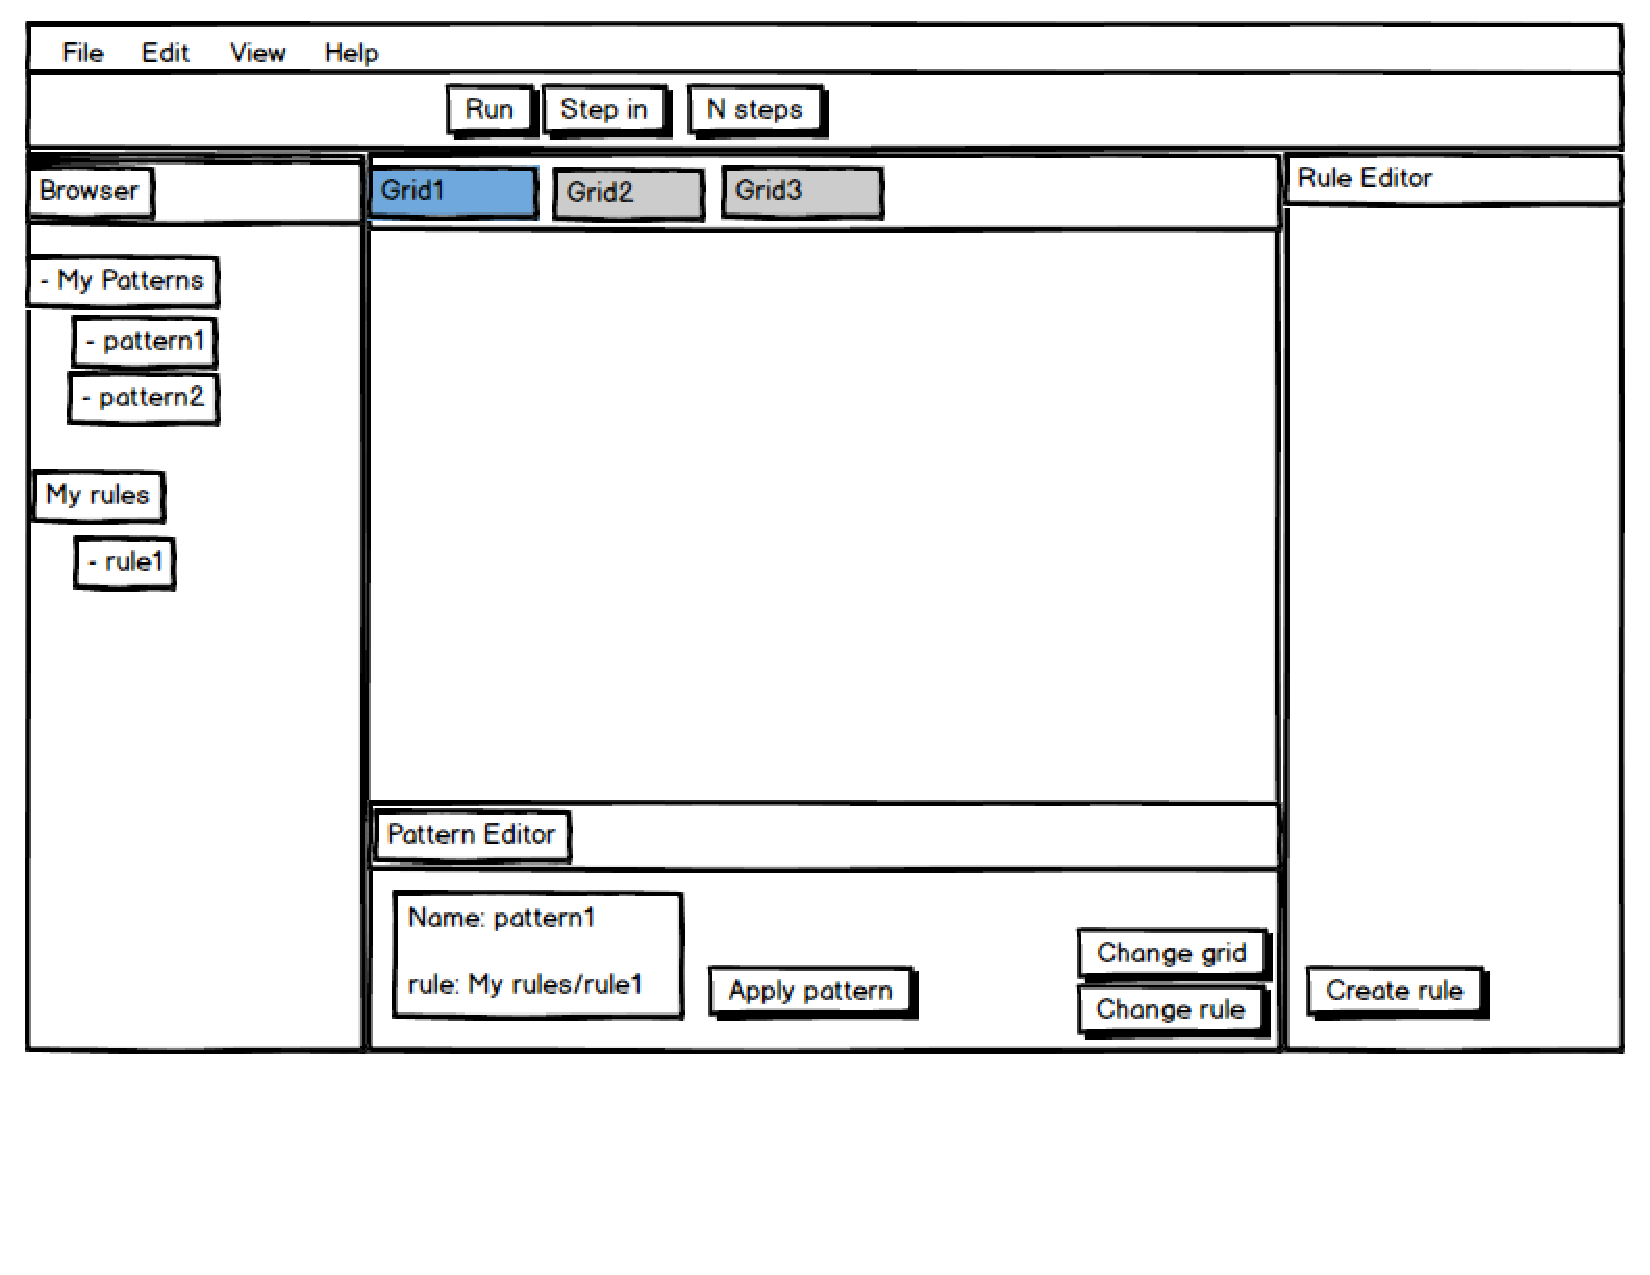
\includegraphics[page=1,width=1.5\textwidth, center]{images/gui_mockup.pdf}
	  \label{fig:gui}
	\end{figure}

	In figure ~\ref{fig:gui} we see an example of components alignment
	

\section{Risk analysis}

The biggest risk of this project is not finishing the application in time.
The developer should make sure that all requirements of highest priority are implemented
first.


\end{document}
